\documentclass[xcolor=dvipsnames]{beamer} 
\usetheme{umbc1} 
\usepackage{textpos,fancyvrb}
\usepackage{amsmath}
\usepackage{graphicx}
\usepackage{color, colortbl}
\usepackage{multirow} 
\usepackage{booktabs,xcolor,siunitx}
\usepackage[framemethod=tikz]{mdframed}
\usepackage{caption}
\usepackage[scale=2]{ccicons}
\usepackage[Q=yes]{examplep}
\usepackage[ddmmyyyy]{datetime}
\usepackage{tabu}
\usepackage{textcomp}
\usepackage{ragged2e}
\usepackage{hyperref}
\hypersetup{
colorlinks=false,     
}
\usepackage[T1]{fontenc}
\usepackage{concmath}
\setbeamertemplate{caption}[numbered]




\definecolor{gold}{rgb}{0.85,.66,0}
 \definecolor{khaki}{rgb}{0.941176,0.901961,0.549020}
\definecolor{saffron}{rgb}{0.96, 0.77, 0.19}
\definecolor{sand}{rgb}{0.76, 0.7, 0.5}
\definecolor{ablue}{rgb}{0.94, 0.97, 1.0}
\definecolor{cgreen}{rgb}{0.0, 0.42, 0.24}


\begin{document}
\vspace{-2cm}
\title[Workshop \LaTeX{}]{\textbf{Workshop on\\``Document typesetting and Processing using \LaTeX{}''} \vspace{-0.5cm}}

\author[\today, \ccby{} P. K. Yadav \&  K. Kumar]{\textbf{\vspace{-0.5cm}Session: Your first \LaTeX{} document}}
\institute{\href{http://www.texample.net/tikz/examples/pascals-triangle-and-sierpinski-triangle/}{

\includegraphics[scale=0.2]{fig/cover}}\centering\\
\begin{flushleft}
Presented by: \textbf{P.K. Yadav \& K. Kumar} \\
\hspace{1.85cm}\textbf{Department of Civil Engineering} \hspace{2.5 cm} \today
\end{flushleft}
}         

\date{}




%\titlegraphic{
\includegraphics[width=4cm]{logo}\hspace*{4.75cm}}

%\setcounter{framenumber}{0}

%\logo{
\includegraphics[width=1.5cm,height=1.5cm,keepaspectratio]{logo}}

%\maketitle

{
\setbeamertemplate{footline}{} 
\begin{frame}
\begin{textblock*}{50cm}(0\textwidth,0cm)
%\begin{textblock*}{120mm}(.75\textwidth,-1.5cm)

\includegraphics[width=5cm]{fig/logofinal}
\end{textblock*}
\vspace{1.2cm}


  \titlepage
\end{frame}
}
\addtocounter{framenumber}{-1}
\logo{
\includegraphics[width=1.0cm,height=1.0cm,keepaspectratio]{fig/mujlogo4}}

\section{Conventions}
\begin{frame}{\textbf{\LaTeX{} Conventions I}}

Before we start with document, let us learn \LaTeX{} conventions: First with \underline{\textbf{characters}}\\
\vspace{0.5cm}
\begin{center}

{\small
\setlength{\arrayrulewidth}{0.5pt}
\arrayrulecolor{saffron}
\begin{tabu}to\linewidth{|X[-2.5,c,m]|X[l,m]|}
\arrayrulecolor{gold}\hline

\rowcolor{ablue}
\textcolor{blue}{$\mathbf{\backslash}$} & escape character, \LaTeX{} functions or control sequences start with this character,
\Q{\\alpha, \\section,\\bf, etc.} \\
\arrayrulecolor{gold}\hline

\rowcolor{gray!40}
\textcolor{blue}{\#} & parameter character used in \LaTeX{} macros \\

\arrayrulecolor{gold}\hline

\rowcolor{ablue}
\textcolor{blue}{\$} & math shift character, i.e., \textcolor{blue}{\$} character starts math mode and the next \textcolor{blue}{\$} character stops it\\

\arrayrulecolor{gold}\hline

\rowcolor{gray!40}
\textcolor{blue}{\%} & comment character, \LaTeX{} will ignore the characters after \textcolor{blue}{\%} till the end of that
line \\

\arrayrulecolor{gold}\hline

\rowcolor{ablue}
\textcolor{blue}{\^{}} & superscript character in math, e.g., \Q{ $a^2$} = $a^2$ 
\\

\arrayrulecolor{gold}\hline

\rowcolor{gray!40}
\textcolor{blue}{\_{}} & superscript character in math, e.g., \Q{ $a_2$} = $a_2$  \\

\arrayrulecolor{gold}\hline

\rowcolor{ablue}
\textcolor{blue}{\{} & group open character used to open a local group 
\\

\arrayrulecolor{gold}\hline

\rowcolor{gray!40}
\textcolor{blue}{\}} & group open character used to close a local group 
\\

\arrayrulecolor{gold}\hline

\rowcolor{ablue}
\textcolor{blue}{$\tilde{}$} & unbreakable space
\\

\arrayrulecolor{gold}\hline

\end{tabu}
}

\end{center}

\end{frame}

\begin{frame}[fragile]{\textbf{\LaTeX{} Conventions II}}

\textcolor{blue}{Alphabets and numerals}\\

\vspace{0.2cm}
Alphabets and numerals other than what listed in the last slide are entered as in any other program or word processor.\\

\vspace{0.5cm}
\textcolor{blue}{Mathematical symbols and notations}

\vspace{0.2cm}

\justifying
Greek letters, various math operators including negated operators, arrows, stretchy delimiters, etc.,  are normally a coded as command. For e.g. for Greek alpha character we use 
\textcolor{blue}{\textbackslash alpha} to produce \textcolor{blue}{$\alpha$}.\\

\vspace{0.2cm}
To produce \fbox{$\alpha^2+\beta^2 = 0$} we use:\\
%\framebox{

%}

\begin{center}

\begin{minipage}{5cm}
\begin{Verbatim}[frame=single]
\begin{equation}
\alpha^2+\beta^2 = 0
\end{equation}
\end{Verbatim}
\end{minipage}

\end{center}

\end{frame}


\begin{frame}[fragile]{\textbf{\LaTeX{} Conventions III}}

\textcolor{blue}{More Mathematical symbols and notations}\\
\vspace{0.2cm}
\justifying
Similarly, a wide variety of symbols are accessed with names similar to what we ordinarily
denote them. For instance, \textcolor{red}{$\swarrow$, $\psi$,
$\longrightarrow$, $\sum$, $\subseteq$, $\not\subseteq$} are generated with \textcolor{red}{\textbackslash swarrow, \textbackslash psi,
\textbackslash longrightarrow, \textbackslash sum, \textbackslash subseteq, \textbackslash not\textbackslash subseteq}.\\
\vspace{0.2cm}

\textcolor{blue}{Accented characters}\\

\vspace{0.2cm}

Languages other than English have a variety of accents and special symbols. See this sentence:
\begin{center}
El se\~nor est\'a bien, gar\c{c}on, \'El est\'a aq\"u\'{\i}
\end{center}


is generated by:\\

\vspace{0.2cm}

\begin{minipage}{11.1cm}
\small
\begin{Verbatim}[frame=single]
El se\~nor est\'a bien, gar\c{c}on, \'El est\'a aq\"u\'{\i}
\end{Verbatim}
\end{minipage}


\end{frame}


\section{First \LaTeX{} code}

\begin{frame}[fragile]{\textbf{The first \LaTeX{} code I- The document format}}

 
Any \LaTeX{} specifier (or Keyword, or function) consist of\par
\vspace{0.2cm}
\textcolor{red}{$\textrm{KEYWORD}$$[\textrm{options in square bracket}]$$\{\textrm{Argument in Braces}\}$.}\\
 \vspace{0.2cm}
 Let us start with out first \LaTeX{} code and document.\\
 \vspace{0.4cm}

\begin{columns}
\begin{column}{0.5\textwidth}
The \LaTeX{} document starts with \textcolor{red}{PREAMBLE} - the document format\\

 \vspace{0.2cm}
The first Premable specifier : \textcolor{red}{DOCUMENTCLASS} with argument- usually ARTICLE, BOOK, REPORT, LETTER etc.\\

 \vspace{0.2cm}

Standard format can be modified by- \textcolor{red}{USEPACKAGE} specifier.\\

\end{column}
\hfill
\begin{column}{0.57\textwidth}
\small
\begin{Verbatim}[frame=single]

% This is Preamble

\documentclass[a4paper, 11pt]
{article}
\usepackage{graphicx}
\usepackage{amsmath}
%amsmath is the package name


\end{Verbatim}
\end{column}
\end{columns}



\end{frame}

\begin{frame}[fragile]{\textbf{The first \LaTeX{} code II- The front-matter}}



The Preamble is followed by the code \textcolor{red}{$\backslash$begin\{document\}}, 
which is closed at the end of the document with \textcolor{red}{$\backslash$end\{document\}}.\\

 \vspace{0.2cm}
\begin{columns}
\begin{column}{0.4\textwidth}


We start with \textbf{`front page specifiers'}. \\
 \vspace{0.2cm}
 
We use specifiers e.g.
  \textcolor{red}{$\backslash$title\{\},  
  $\backslash$author\{\}, $\backslash$date\{\}} etc.\\
  
   \vspace{0.4cm}
The command  \textcolor{red}{$\backslash$maketitle} compiles the front-matters.

\end{column}

\begin{column}{0.5\textwidth}
\small
\begin{Verbatim}[frame=single]

% These are front-matters

\title{Your title goes here}
\author{Auth1 \and Auth.2
 \\Affili.}
\date{\today}

\maketitle

\end{Verbatim}
\end{column}


\end{columns}


\end{frame}

\begin{frame}[fragile]{\textbf{The first \LaTeX{} code III- The document body}}

\begin{columns}
\begin{column}{0.4\textwidth}

As can be expected, the document body specifier are:\\
  
   \vspace{0.3cm}

\textcolor{red}{$\backslash$begin\{abstract\}} and ends with \textcolor{red}{$\backslash$end\{abstract\}}- here \textcolor{red}{abstract} is called the \textbf{environment}.\\
   \vspace{0.3cm}
   
Other specifier are: \textcolor{red}{$\backslash$keywords}, \textcolor{red}{$\backslash$section\{\}}, \textcolor{red}{$\backslash$subsection\{\}},
\textcolor{red}{$\backslash$subsubsection\{\}}, etc.

\end{column}

\begin{column}{0.5\textwidth}
\small
\begin{Verbatim}[frame=single]

% These are front-matters

\begin{abstract}
Your abstract goes here.
\end{abstract}

\section{Introduction}
\subsection{Actual Problem}
\subsubsection{Case-Study}

\section{Experiment}
\section{Discussions}
\section{Conclusions}

\end{Verbatim}
\end{column}

\end{columns}

\end{frame}

\section{Listing Environment}
\begin{frame}[fragile]{\textbf{The first \LaTeX{} code V- The Lists Environment}}



Normally, \textbf{Acknowledgements}, \textbf{Appendices} and \textbf{References} make the end-matters. In \LaTeX{} we specify them as:\\
\vspace{0.4cm}

\begin{columns}
\begin{column}{0.5\textwidth}

Appendices and Acknowledgements can be coded as: \textcolor{red}{$\backslash$section\{Acknowledgement\}} and \textcolor{red}{$\backslash$section\{Appendices\}}.\\
\vspace{0.2cm}

For References we use \textbf{thebibliography} environment, as:
\textcolor{red}{$\backslash$begin\{thebibliography\}} and ends with \textcolor{red}{$\backslash$end\{thebibliography\}}.\\
\vspace{0.2cm}

 The actual references are then coded with specifier:
 \textcolor{red}{$\backslash$bibitem\{ref. label\}\{ref. detail\}}

\end{column}


\begin{column}{0.52\textwidth}
\small

\begin{Verbatim}[frame=single]
% These are end-matters

\section{Appendices}
\section*{Acknowledgements} 
%*puts off the section number

\begin{thebibliography}{99}
\bibitem{Stump}{D. R. Stump,
 ``How to write a LaTeX 
 paper'', 2000.}
\end{thebibliography}
\end{Verbatim}

\end{column}

\end{columns}

\end{frame}


\begin{frame}[fragile]{\textbf{The first \LaTeX{} code V- The Lists Environment}}



Scientific documents normally contains \textbf{Lists, Figures, Tables, Equations (Maths \& Chemistry) and References}. We will learn to include these in our document.\\
\vspace{0.2cm} 

We start with the \textcolor{red}{\textbf{Lists}}. \\
\vspace{0.2cm} 

Normally following two lists are used:\\
\vspace{0.2cm} 

\textcolor{red}{$\backslash$begin}{\textcolor{red}{\{enumerate\}}} \hspace{0.3cm}list text \hspace{0.3cm} \textcolor{red}{$\backslash$end}{\textcolor{red}{\{enumerate\}}}\\
\vspace{0.2cm}

\textcolor{red}{$\backslash$begin}{\textcolor{red}{\{itemize\}}} \hspace{0.83cm}list text \hspace{0.5cm} \textcolor{red}{$\backslash$end}{\textcolor{red}{\{itemize\}}}
\\
\vspace{0.2cm}
The list text is coded as \textcolor{red}{$\backslash$item}.\\
\vspace{0.05cm}.

\begin{minipage}{10cm}
\begin{Verbatim}[frame=single]
\begin{enumerate}
\item The labels consists of sequential numbers.
\item The numbers starts at 1 with every call
 to the enumerate environment.
\end{enumerate}
\end{Verbatim}
\end{minipage}


\end{frame}

\begin{frame}[fragile]{\textbf{The first \LaTeX{} code V- The Lists}}



Quite often we use a list within a list, i.e. the nested list. These are very simple. We use both \textbf{itemize} and \textbf{enumerate} environments for our example. \\

\vspace{0.2cm}

\renewcommand\theenumii{\alph{enumii}}
\begin{enumerate}
\item The {\tt itemize} label at the first level is a bullet.
\begin{itemize}
\item The numbering is with Arabic numerals since this is ...
\begin{enumerate}
\item This is the third level of the nesting, but the ...
\item The label at this level is a long dash.
\end{enumerate}
\item Every list should contain at least two points.
\end{itemize}
\item Blank lines ahead of an ...\\
\vspace{0.2cm}
\end{enumerate}

\tiny 
\begin{minipage}{8cm}
\begin{Verbatim}[frame=single]
\begin{enumerate}
\item The {\tt itemize} label at the first level is a bullet.
\begin{itemize}
\item The numbering is with Arabic numerals since this is ...
\begin{enumerate}
\item This is the third level of the nesting, but the ...
\item The label at this level is a long dash.
\end{enumerate}
\item Every list should contain at least two points.
\end{itemize}
\item Blank lines ahead of an ...\\
\vspace{0.2cm}
\end{enumerate}
\end{Verbatim}
\end{minipage}


\end{frame}

\begin{frame}[fragile]{\textbf{The first \LaTeX{} code VI- The Figure Environment}}


\justifying

Figures are normally created in different software, e.g. MS Excel$^\circledR{}$, and then attached (pasted)  to the document. This is similar in \LaTeX{}.\\

\vspace{0.2cm}

\textbf{CAPTION} and \textbf{Figure Number} are part of figure in any scientific document. Eventually, it may be desired to obtain\textbf{ Table of Figures}. In \LaTeX{} entire work with figure is rather simple after we add in the preamble: \textcolor{red}{$\backslash$usepackage\{graphicx\}}\\

\vspace{0.2cm}

To insert a figure the \textbf{figure} environment is used, as:\\

\vspace{0.3cm}


\begin{minipage}{8cm}
\begin{Verbatim}[frame=single]
\begin{figure}[Position]
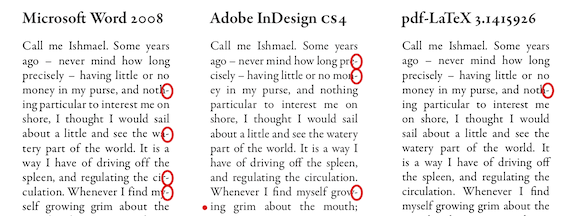
\includegraphics[Figure size]{fig1.jpg}
\caption{figure title}
\end{figure}
\end{Verbatim}
\end{minipage}

\vspace{0.3cm}
\normalfont
\textbf{Let us learn the code in detail.}

\end{frame}

\begin{frame}[fragile]{\textbf{The first \LaTeX{} code VII- The Figure Environment}}


\justifying

First the figure environment \\

\vspace{0.1cm}
\begin{center}
\begin{minipage}{6cm}
\color{red}\begin{Verbatim}[frame=single]
\begin{figure}[Position]
\end{figure}
\end{Verbatim}
\end{minipage}
\end{center}

\vspace{0.1cm}
The \textbf{POSITION} option specifies where in the page the figure should be attached- i.e. \textcolor{red}{\textbf{h}} - here, where the code is placed, \textcolor{red}{\textbf{b}} - at the \textbf{bottom} of the page, \textcolor{red}{\textbf{t}} - at the \textbf{top} of the page, \textcolor{red}{\textbf{!}} - for overriding the \LaTeX{} internal code. \\

\vspace{0.3cm}

The \textbf{POSITION} can also be specified as a combination, e.g. \textcolor{red}{\textbf{htb}}.

\vspace{0.3cm}
\begin{center}
\begin{minipage}{6cm}
\color{red}\begin{Verbatim}[frame=single]
\begin{figure}[h]
\end{figure}
\end{Verbatim}
\end{minipage}
\end{center}


\end{frame}


\begin{frame}[fragile]{\textbf{The first \LaTeX{} code VIII- The Figure Environment}}


\justifying

Next we include the figure with\\

\vspace{0.1cm}
\begin{center}
\begin{minipage}{8cm}
\color{red}\begin{Verbatim}[frame=single]
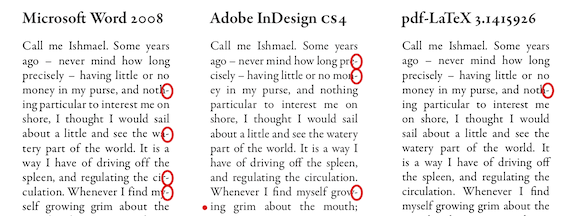
\includegraphics[Figure size]{fig1.jpg}
\end{Verbatim}
\end{minipage}
\end{center}

\vspace{0.1cm}
Several figure formats such as, \textcolor{red}{\textbf{EPS, PDF, JPG, BMF, PNG}} can be attached to the \LaTeX{} document. These formats can be obtained from any standard mathematical analysis software. \\

\vspace{0.1cm}

The power of \LaTeX{} is more on the \textbf{size and orientation} option of the \textcolor{red}{$\backslash$includegraphics} specifier.\\

\vspace{0.3cm}

The option: \textcolor{red}{\textbf{angle=xx}}, where xx specifies angle in degrees- e.g. 45, 130 etc. can be used to rotate the figure.


\end{frame}

\begin{frame}[fragile]{\textbf{The first \LaTeX{} code IX- The Figure Environment}}


\justifying

Figure sizing options are: \textcolor{red}{\textbf{width=xx, height=xx, scale=xx, keepaspectratio}}, where \textbf{`xx'} refers to dimension, e.g. 4cm, 10mm, 3in, 12pt etc. for the width and height, whereas it is a number for scale.\\

\vspace{0.4cm}

A combination of several options, e.g. [scale= 0.1, angle=123.4 ], can be used for the figure.\\

\vspace{0.4cm}
Lastly, we put caption using  \textcolor{red}{$\backslash$caption\{\}} specifier. Caption is place below the figure in the document, so we have to place caption specifier below the \textcolor{red}{$\backslash$includegraphics\{\}} specifier.

\end{frame}

\begin{frame}[fragile]{\textbf{The first \LaTeX{} code X- The Figure Environment}}


\justifying
\fbox{
\begin{minipage}{0.3\linewidth}
\begin{figure}[h]

\includegraphics[scale=0.2]{fig/logo} %\centering
\caption{scale = 0.2}
\end{figure}
\end{minipage}
}
\hfill
\fbox{
\begin{minipage}{0.5\linewidth}
\begin{figure}[h]

\includegraphics[scale=0.2, height=0.3in, angle= 120]{fig/logo} %\centering
\caption{scale = 0.2, height= 0.3in, angle= 120}
\end{figure}
\end{minipage}
}

\vfill

\fbox{
\begin{minipage}{0.6\linewidth}
\begin{figure}[h]

\includegraphics[width= 5cm, angle= 180]{fig/logo} %\centering
\caption{width= 5cm, angle= 180}
\end{figure}
\end{minipage}
}


\end{frame}

\section{Conclusion}
\begin{frame}{\textbf{Concluding Remarks}}
\justifying
As stated, \LaTeX{} is highly customizable, but for that we need to additional \textbf{packages} in our preamble. There are over 1000 packages available.\\

\vspace{0.4cm}

Normally the publishers provide their template which include all additional packages.\\

\vspace{0.4cm}

Some important packages, that you may check, are: \textcolor{red}{\textbf{color, xcolor, subfigure, subcaption, float, easylist, amssymb, amsmath }}.\\
\vspace{0.3cm}

You may check here for more: \href{http://en.wikibooks.org/wiki/LaTeX/List_Structures}{\textcolor{red}{for Lists}} and \href{http://en.wikibooks.org/wiki/LaTeX/Floats,_Figures_and_Captions}{\textcolor{red}{for Figures}}, \href{http://en.wikibooks.org/wiki/LaTeX/Importing_Graphics}{\textcolor{red}{also here for Figures}}


\end{frame}


{
\setbeamertemplate{footline}{} 
\begin{frame}{\Huge \textbf{Tables, equations $\ldots$,}}
\pagestyle{plain}
\Huge

\textbf{Next, improve our \LaTeX{} document.}


\end{frame}

}

\end{document}
